\documentclass[a4paper,12pt]{article}
\usepackage{amssymb}
\usepackage{amsfonts}

% Кодировка и язык
\usepackage[utf8]{inputenc}
\usepackage[T2A]{fontenc}
\usepackage[russian]{babel}


% Математические пакеты
\usepackage{amsmath,amsfonts,amssymb}
%Таблицы
\usepackage{array}
\usepackage{booktabs} % Для более красивых горизонтальных линий в таблицах
\usepackage{graphicx}
\usepackage{array}
\usepackage{booktabs}
% Геометрия страницы
\usepackage{geometry}
\geometry{top=2cm, bottom=2cm, left=2.5cm, right=2.5cm}
% Гиперссылки (лучше загружать последним)
\usepackage{hyperref}


% Настройки заголовка
\title{Домашнее задание}
\author{Студент: \textbf{Ростислав Лохов}}
\date{\today}

\begin{document}

% Титульный лист
\begin{titlepage}
    \centering
    \vspace*{1cm}

    \Huge
    \textbf{Домашнее задание}

    \vspace{0.5cm}
    \LARGE
    По курсу: \textbf{Экономика}

    \vspace{1.5cm}

    \textbf{Студент: Ростислав Лохов}

    \vfill

    \Large
    АНО ВО Центральный университет\\
    \vspace{0.3cm}
    \today

\end{titlepage}

% Содержание
\tableofcontents
\newpage

% Основной текст
\section{Сине-Красный уровень}

\subsection{Задача 1}
\begin{enumerate}
    \item Уменьшению
    \item Уменьшением
    \item Уменьшению, увеличению
    \item 90, 95
    \item -15, -15
    \item ростом
    \item увеличится
\end{enumerate}

\subsection{Задача 2}
\begin{enumerate}
    \item ВВП (Y) = 5900, Потребительские расходы (C) = 3000, Государственные закупки (G) = 1500, Налоги (T) = 2100, Трансферты (TR) = 500.
    \item Чистые налоги = налоги - трансферты = 1600
    \item Распологаемый доход = ВВП - чистые налоги = 4300
    \item Частные сбережения = распологаемый доход - потребление = 1300
    \item Сальдо = налоги - госзакупки - трансферты = 100
\end{enumerate}

\subsection{Задача 3}
\begin{enumerate}
    \item Из за воздержания от посещения публичных мест сокращаются потребительские расходы
    \item Т.к потребительские расходы являются крупнейшим компонентом совокупных расходов, то их падение ведет к уменьшению совокупных расходов.
    \item Т.к совокупные расходы равны совокупным доходам, то их падение ведет к уменьшению совокупных доходов.
    \item Снижение совокупных доходов ведет к сокращению потребительских расходов и к уменьшению налоговых поступленй.
\end{enumerate}

\subsection{Задача 4}
\begin{enumerate}
    \item Более высокое экономическое развитие страны = лучше уровень жизни (жилье, еда, доступ к благам). Сравнение условных Мали (низкий), Мексики (средний), Швеции (высокий) показывает эту прямую зависимость.
\end{enumerate}

\subsection{Задача 5}
\begin{enumerate}
    \item Сальдо гос бюджета = T-G=2000-1500-700=-200 - дефицит
    \item Сальдо торг баланса = X-IM = 800-900=-100 - дефицит
    \item ВВП = C+I+G+NX = 2050+1050+1500-100=4600
    \item Распологаемый доход 4600-2000=3300
    \item Иньекции = I+G+X = 1050+1500+800=3350
    \item Утечки = T-TR+IM = 1150+2000-700+900=3350
    \item Инвестиции = частные сбережение + сальдо гос + сальдо тор = 1050 = 1050 - баланс соблюдается
\end{enumerate}

\section{Черный уровень}
\subsection{Задача 1}
\begin{enumerate}
    \item X=500, IM=600, Sp=1000, I=400, G=350, Tr=200, Tf=500
    \item Дефицит бюджета=50, Профицит торг. баланса (NX)=100, Сумма инъекций (J)=1450
    \item Значения X и IM с диаграммы дают NX = 500 - 600 = -100 (дефицит) что противоречит условию профицита NX=100. Следовательно, ошибка в X или IM
    \item Если ошибка в X (X=700, IM=600 для NX=100) то J=1650 (не равно 1450)
    \item Если ошибка в IM (IM=400, X=500 для NX=100) то J = 400+350+500+200 = 1450 (совпадает)
    \item Дефицит = G + Tr - T = 50. T = Th + Tf = Th + 500. => 350 + 200 - (Th + 500) = 50 => Th = 0. Общие налоги T=500
    \item Единственная ошибка на диаграмме позволяющая удовлетворить всем трем числовым условиям (NX=100, J=1450, Дефицит=50) это значение Импорта (IM) Оно должно быть 400 вместо 600
    \item Поток РТУ -> ВМ = 400
    \item Поток Домашние хозяйства -> Государство (Th) = 0
    \item Остальное невозможно
    \item Sg (Государственные сбережения): Sg = T - G - Tr = 500 - 350 - 200 = -50. Направление - от финансового рынка к государству, величина 50
    \item Sf (Иностранные сбережения): Sf = IM - X = 400 - 500 = -100. Направление - от финансового рынка к внешнему миру, величина 100.
\end{enumerate}

\subsection{Задача 2}
\begin{enumerate}
    \item Кто приносит деньги на фин рынок США? Домохозяйства и внешний мир. Берет - Фирмы и гос-во
    \item Макроэкономические уязвимости - уязвимость от иностранного капитала, рост госдолга и внешнего долга
    \item Проще говоря - прекращение притока всех иностранных капиталов, смена резервной валюты в мире, спровоцирует сильнейший экономический кризис. США давно уже не выигрывают т.к производить внутри страны стало невероятно дорого, из за чего все производства ушли в другие страны, пытался Байден фиксить данную проблему субсидиями для заводов, особо не помогло. Заводы новые есть, производить стало дорого. Пришёл Трамп - в пятницу устроил веселье - ввел пошлины на всех, для того, чтобы в остальных странах производить стало невыгодно.
\end{enumerate}

\subsection{Задача 3}
\begin{enumerate}
    \item Дефицит: 2020, 2022, 2023, 2024
    \item Профицит  2019, 2021\dots
    \item  Дефициты связаны с пандемией, падением нефтегазовых доходов и ростом расходов (социальных, оборонных:), экономических). Профициты – с высокими ценами на нефть/газ
    \item Доля нефтегазовых доходов, с 50 процентов до менее чем 30 к 2027 году.
    \item Снижение доли нефтегазовых доходов снижает зависимость от курса нефти.
    \item Основные налоговые поступления - НДС и НДПИ. Что то конкретное про изменения сказать сложно
    \item Основные статьи - Соц политика, нац оборона, нацбезопасность, нацэкономика
    \item С 2022 года рост статьи нац оборона.
    \item 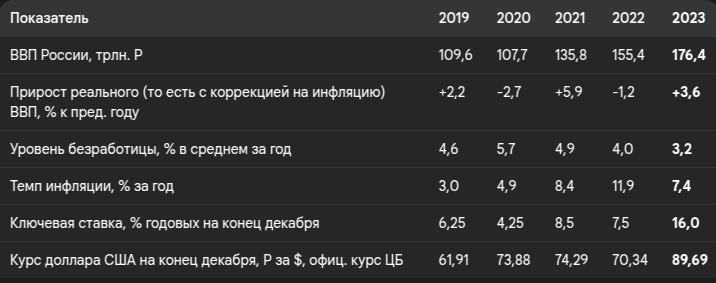
\includegraphics[scale=0.45]{graphs/9.1.png}
\end{enumerate}


\end{document}